\documentclass[12pt]{report}
    \title{\textbf{CAP4630 Intro to Artificial Intelligence \\ Knowledge-based
Intelligent System \\ Project 3 - Report}}
    \author{Tobias Dault, Eyob Tekle, William L. Thomson Jr.}
    \date{April 1st, 2022}

    \addtolength{\textheight}{3cm}
	\usepackage{enumitem}
    \usepackage{hyperref}
    \usepackage{float}
    \usepackage{graphicx}
    \usepackage{multicol}
    \usepackage{subcaption}
    \usepackage[tmargin=1in,lmargin=1in,rmargin=1in]{geometry}
	\usepackage{titlesec}
	
    \DeclareCaptionFormat{custom}
    {%
        \textbf{\footnotesize #1#2}\textit{\footnotesize #3}
    }
    \captionsetup{format=custom}

    \graphicspath{ {./assets/} }

	\hypersetup{ colorlinks=true, linkcolor=blue, filecolor=purple, urlcolor=cyan }

    \newlength\tindent
    \setlength{\tindent}{\parindent}
    \setlength{\parindent}{0pt}
    \renewcommand{\indent}{\hspace*{\tindent}}

    \setlist[description]{noitemsep, topsep=0pt, itemsep=.5em}
    \setlist[enumerate]{noitemsep, topsep=0pt, itemsep=.5em}
    \setlist[itemize]{noitemsep, topsep=0pt, itemsep=.5em}

    \titleformat{\chapter}
	{\Large\bfseries}
	{\thechapter.}{0.5em}{}

	\titleformat{\section}
	{\large\bfseries}
	{\thesection.}{0.5em}{}

	\titleformat{\subsection}
	{\normalsize\bfseries}
	{\thesubsection.}{0.5em}{}

    \titlespacing\chapter{0pt}{12pt plus 0pt minus 4pt}{0pt plus 0pt minus 4pt}
    \titlespacing\section{0pt}{12pt plus 4pt minus 8pt}{0pt plus 2pt minus 8pt}
    \titlespacing\subsection{0pt}{12pt plus 4pt minus 2pt}{0pt plus 2pt minus 2pt}

\begin{document}

\maketitle
\tableofcontents
\thispagestyle{empty}

\chapter{Overview}
\section{About}
This program is a knowledge-based intelligent system that collects user preferences and reasons about them. The program collects names of attributes, values of attributes ($A$), hard constraints represented as propositional formulas in conjunctive normal form (CNF) ($H$), and preferences languages of penalty logic, possibilistic logic, and qualitative choice logic with preference formulas ($T$) also in conjunctive normal form (CNF) from user input or files with the purpose of performing the following four reasoning tasks: \\

\begin{description}[style=multiline,leftmargin=12em]
  \item [Existence of Feasible Objects] Whether there are feasible objects w.r.t $H$,
that is, whether there are models of $H$ that are truth assignments making $H$ true.
  \item [Exemplification] Generate two random feasible objects, and show the preference between the two (strict preference or equivalence) w.r.t $T$
  \item [Optimization] Find an optimal object w.r.t $T$
  \item [Omni-Optimization] Find all optimal objects w.r.t $T$
\end{description}

\section{Design}
The program is written in Python and leverages the Tkinter python binding to TK GUI toolkit, used for the GUI of the program. The underlying logic is mostly performed with the use of clasp, an answer set solver for normal and disjunctive logic programs. The program wraps the clasp binary and uses it to perform tasks such as existence of feasible objects and for penalty and possibilistic preference logics. Qualitative choice logic is performed internally in the programs code without the use of clasp.

\subsection{Clasp}
The use of clasp in the program is done via the python subprocess where data is piped to clasp via stdin and piped back from clasp via stdout. Once inputted or loaded from file, the attributes are stored in a dictionary with the key being the numerical clasp format of positive and negative integers starting at 1/-1 up to $n$ attributes, based on the number that were inputted or loaded from file. Hard constraints, penalty logic preferences, and possibilitistic logic preferences are converted to clauses in clasp numerical format, the attributes' dictionary keys, that are obtained from the dictionary using the text values of each attribute's option. Likewise, when processing output from clasp, the keys are used to obtain the text value from the attributes dictionary. This allows for mapping between the clasp numerical format and the human readable attribute options.

\newpage
\subsection{Feasible Objects}
Feasible objects are identified by passing all the hard constraints to clasp as clauses in clasp numerical format, and obtaining the set of objects returned from clasp. The result is stored in a dictionary for use by other functions, with the object number as they key, and clasp and human readable data stored as values. The results are also displayed in a table on the output tab with both the numerical clasp format and the human readable attribute options, along with object number that is used within the program to refer to specific objects for the various output tables, preference logic, optimal, and exemplification tables.

\subsection{Exemplification}
Exemplification of two random feasible objects is performed as a series of calls to clasp, with added logic, and processing portions of that data. Along with some internal handling of qualitative comparisons that are done without the use of clasp. Exemplification invokes the feasibility functionality, and builds upon it. The bulk of all task functionality is done as part of the exemplification function. Exemplification functionality provides the foundation that other optimization tasks utilize.\\

As part of exemplification, each of the penalty and possibilistic logic preferences are converted into clauses in clasp numerical format and added to the hard constraints clauses and passed onto clasp. If the result from clasp contains a feasible object then no penalty is added or tolerance value is assigned. Likewise, if a feasible object is not in the output returned by clasp, then a penalty value is assigned to that objects preferences, or tolerance value subtracted. These resulting values are used in comparing the objects for strict preference or equivalence, and also later on for determining optimal objects. The resulting penalty and tolerance values are stored in value sorted dictionaries with object numbers as indexes, which are used for finding optimal objects for each penalty and possibilistic logic preferences.\\

Also as part of exemplification, for qualitative choice logic, with each iteration of the qualitative choice preferences a satisfaction check is done to ensure the optimal combination of the attributes is made. The first satisfaction check is done in reverse, surveying each object for an implied attribute(s). If the initial check fails, the preference is assigned with the max satisfaction degree of infinity, but if passed, then the second check is designed to look for the best combination of the attributes in each object. The best choices are labeled with the lowest positive integer of 1, and is incremented by 1 with each attribute pairing that the feasible objects fail to meet. If none are satisfied then the preference is assigned with the max satisfaction degree of infinity. These degree counts are used in determining if qualitative objects are preferred over another, equivalent, or incomparable and that information is stored if the objects being processed are currently the two being considered for exemplification. In the process, all optimal qualitative choice objects numbers are stored in a list for use by optimization tasks.\\

The results of exemplification from all three preference logics, penalty, possibilistic, and qualitative are displayed in a table showing which of the two objects being compared and if they are preferred, equivalent, or incomparable for each preference logic.

\newpage
\subsection{Optimization}
With the bulk of the work done, the task of finding optimal objects became rather trivial. For penalty and possibilistic logic finding the optimal objects is simply a matter of returning the first element from dictionaries sorted in ascending order by value for optimal penalty and possibilistic, and returning the first element of a list for optimal qualitative. For optimization, only the first object is returned as a single optimal object from either the penalty and possibilistic dictionaries or qualitative list. For optimal penalty and possibilistic object, the object key is obtained from the first element of the value sorted dictionaries. For optimal qualitative it is simply the first element of the optimal qualitative list. The optimal objects information is retrieved from the feasible objects dictionary and is displayed in the resulting optimal tables for each of the three preference logics penalty, possibilistic, and qualitative.\\

In the event neither feasible objects or exemplification function has been run, optimization will invoke exemplification function which in turn invokes feasible object function to ensure the necessary data structures have been populated for the optimization functionality. 

\subsection{Omni-Optimization}
Like optimization, with the work having been already done, omni-optimization returns all optimal objects from the value sorted optimal penalty and possibilistic logic dictionaries and the optimal qualitative list. Instead of returning a single object from the optimal penalty and possibilistic logic dictionaries and optimal qualitative list like in optimization. For optimal penalty and possibilistic logic dictionaries the elements in value sorted ascending order are iterated until a value changes, indicting the end of the optimal penalty and possibilistic logic objects in each of their respective dictionaries. For optimal qualitative, the optimal qualitative list is iterated through in its entirety because it only has object numbers for optimal qualitative objects. Like optimization, the optimal objects information is retrieved from the feasible objects dictionary and is displayed in the resulting optimal tables for each of the three preference logics penalty, possibilistic, and qualitative.\\

Also like optimization, In the event neither feasible objects or exemplification function has been run, omni-optimization will invoke exemplification function which in turn invokes feasible object function to ensure the necessary data structures have been populated for the omni-optimization functionality. 

\newpage
\section{Operation}
The program is a GUI that is started from a terminal. All that is need to run the program is to have the necessary system requirements, Python $\geq$ 3.9, Tkinter $\geq$ 8.6, Tcl/TK $\geq$ 8.6, and clasp $\geq$ 3.2. The clasp binary must be available via the system PATH variable. To start the program navigate to the directory it was unpacked in and run the following command(s).

\begin{figure}[H]
\begin{center}
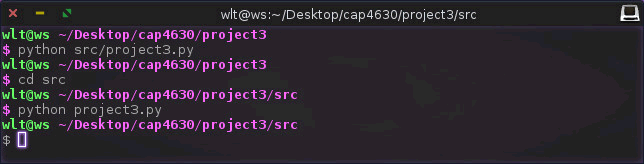
\includegraphics[scale=0.5]{start_program}
\caption{Screenshot of starting the program from a terminal}
\end{center}
\end{figure}

\subsection{Program Start}
Once started you will see the following window appear with input and output tabs.

\begin{multicols}{2}
\begin{figure}[H]
\begin{center}
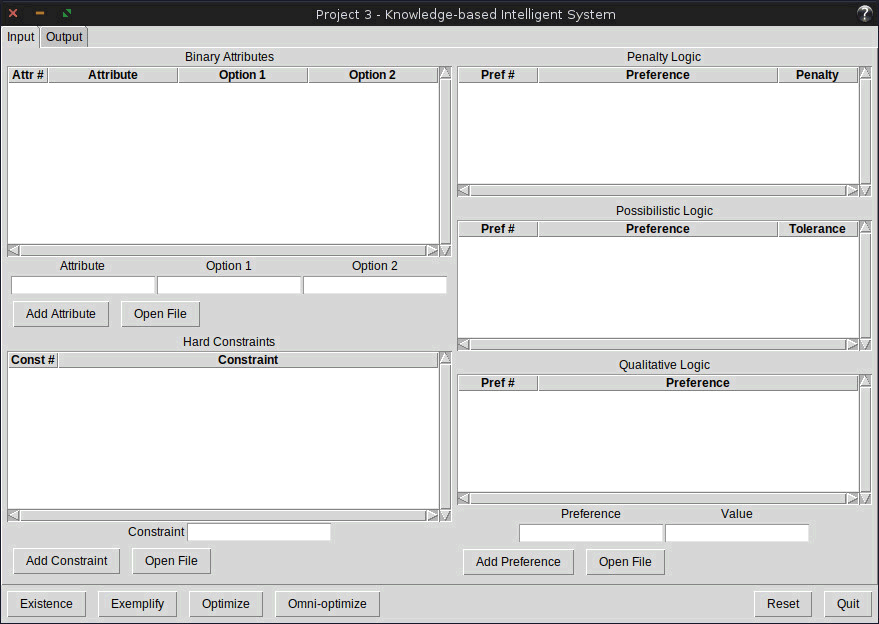
\includegraphics[scale=0.25,trim=1cm 1cm 1cm 1cm]{input_start}
\caption{Screenshot of initial input tab}
\end{center}
\end{figure}
\begin{figure}[H]
\begin{center}
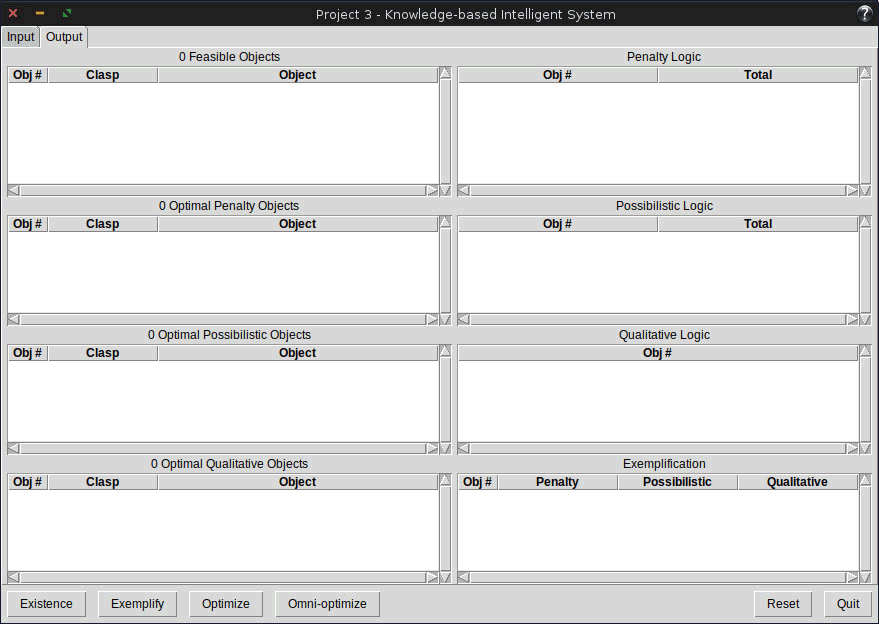
\includegraphics[scale=0.25,trim=1cm 1cm 1cm 1cm]{output_start}
\caption{Screenshot of initial output tab}
\end{center}
\end{figure}
\end{multicols}

The following chapters and sections cover inputting data into the program, generating, and viewing the output.

\chapter{Input}
The program relies upon user input for all functionality, either from direct user input via text input form fields and the add buttons, or by file upload of properly formatted files using the open file buttons, or a combination of user input and file upload. Without such input, the program will not function, and it will prompt the user for missing attributes, hard constraints, and/or preferences before performing any of the intended functions. All input and related actions are performed under the input tab.

\section{Binary Attributes}
The first required program input are the binary attributes. The program requires at least one or more binary attributes to function. Binary attributes can be entered in one by one, or in bulk via a file upload, which is recommended. Additional attributes can be entered directly in addition to those loaded from a file.

\section{Hard Constraints}
The second required program input are the hard constraints. The program requires at least one or more hard constraints to function. Hard constraints can be entered in one by one, or in bulk via a file upload, which is recommended. Additional hard constraints can be entered directly in addition to those loaded from a file.

\section{Preference Logics}
The third and final required program input are the preference logics: penalty logic, possibilistic logic, and qualitative choice logic. The program requires at least one or more preference logics for each of the three types to function. Preference logics can be entered in one by one, or in bulk via a file upload, which is recommended. Additional preference logics can be entered directly in addition to those loaded from a file. The type of logic will be automatically determined based on the value, if one exists, which it does not for qualitative choice logic.

\section{Input Steps and Screenshots}
The following pages contain steps and screenshots showing how to input attributes (names and values), hard constraints, and preference logics from a file into the program. Manual input is not covered, but is only a matter of entering in the information into text fields and pressing the related add buttons.

\newpage
\subsection{Input Binary Attributes from a File}
The following steps are based on using the open file method of inputting attributes.\\

\begin{description}[leftmargin=4em]
\item [Step 1:] Click the \textbf{"Open File"} button below the Binary Attributes table
\begin{figure}[H]
\begin{center}
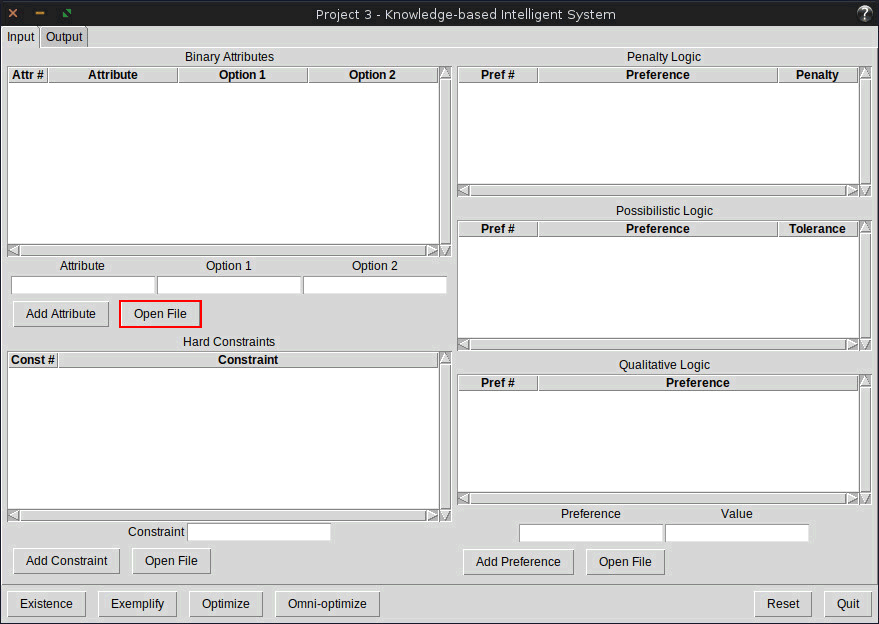
\includegraphics[scale=0.3,trim=1cm 1cm 1cm 1cm]{input_attributes}
\caption{Screenshot of selecting attributes from a file}
\end{center}
\end{figure}
\vspace{-2.5em}
\item [Step 2:] Select the desired file (attributes$\_$test.txt for this example) and click \textbf{"Open"}.
\begin{figure}[H]
\begin{center}
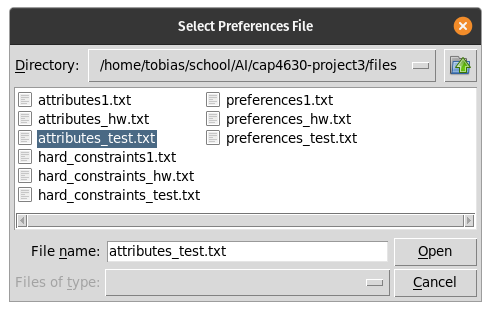
\includegraphics[scale=0.3,trim=1cm 1cm 1cm 1cm]{select_attributes}
\caption{Screenshot of selecting a attributes text file}
\end{center}
\end{figure}
\vspace{-2.5em}
\item [Result:] The contents of the file will be displayed in the \textbf{Binary Attributes table}
\begin{figure}[H]
\begin{center}
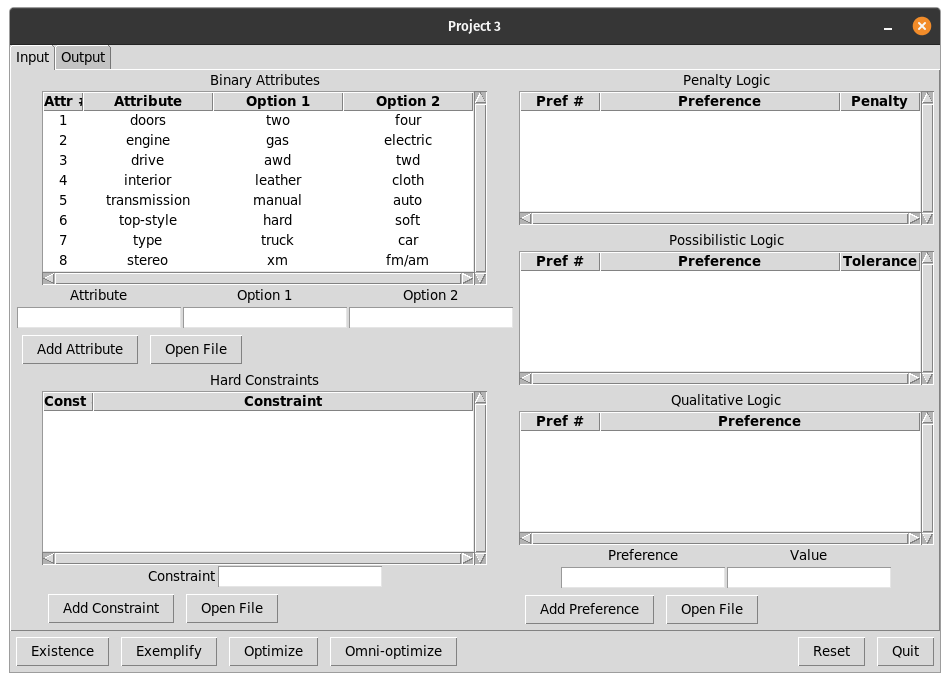
\includegraphics[scale=0.3,trim=1cm 1cm 1cm 1cm]{attributes_imported}
\caption{Screenshot of attributes loaded from file}
\end{center}
\end{figure}
\vspace{-2.5em}
\end{description}


\newpage
\subsection{Input Hard Constraints from a File}
The following steps are based on using the open file method of inputting hard constraints.\\

\begin{description}[leftmargin=4em]
\item [Step 1:] Click the \textbf{"Open File"} button below the Hard Constraints table
\begin{figure}[H]
\begin{center}
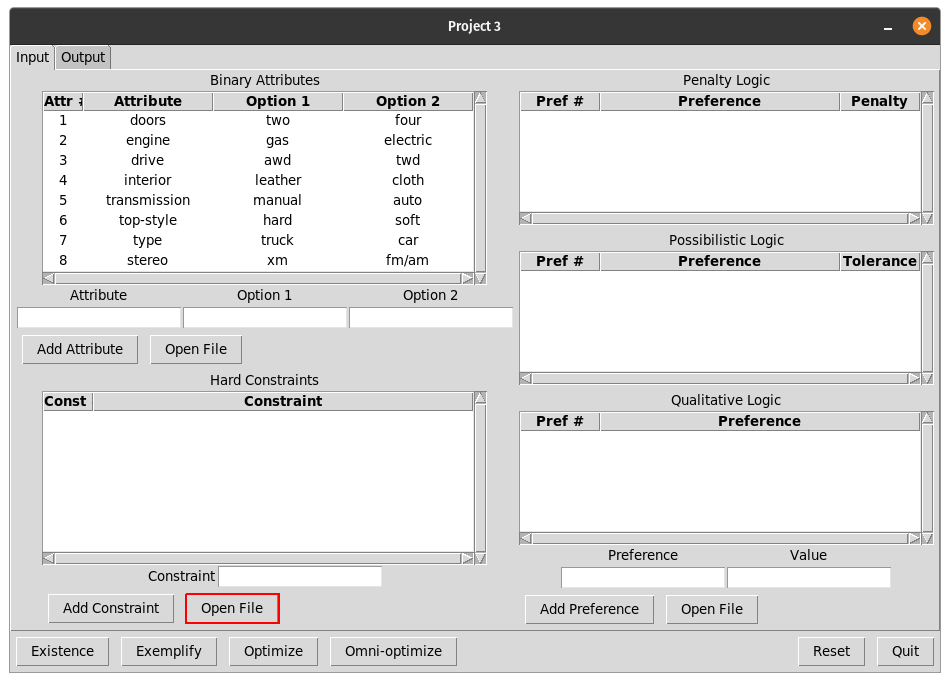
\includegraphics[scale=0.3,trim=1cm 1cm 1cm 1cm]{input_constraints}
\caption{Screenshot of selecting hard constraints from a file}
\end{center}
\end{figure}
\vspace{-2.5em}
\item [Step 2:] Select the desired file (hard$\_$constraints$\_$test.txt for this example) and \textbf{"Open"}.
\begin{figure}[H]
\begin{center}
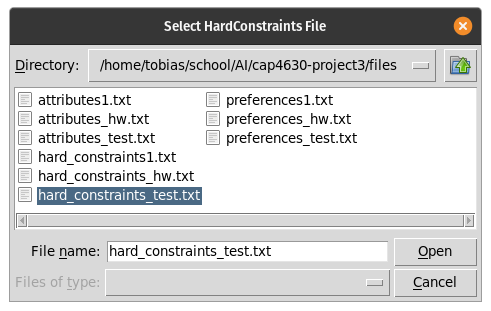
\includegraphics[scale=0.3,trim=1cm 1cm 1cm 1cm]{select_constraints}
\caption{Screenshot of selecting a hard constraints text file}
\end{center}
\end{figure}
\vspace{-2.5em}
\item [Result:] The contents of the file will be displayed in the the \textbf{Hard Constraints table}
\begin{figure}[H]
\begin{center}
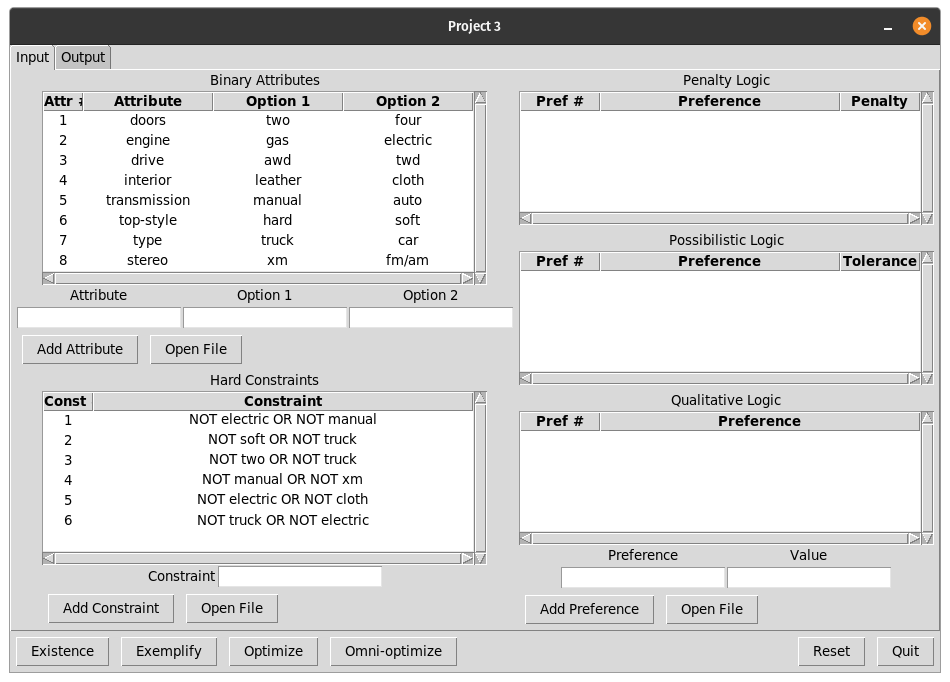
\includegraphics[scale=0.3,trim=1cm 1cm 1cm 1cm]{constraints_imported}
\caption{Screenshot of hard constraints loaded from file}
\end{center}
\end{figure}
\vspace{-2.5em}
\end{description}

\newpage
\subsection{Input Preference Logics from a File}
The following steps are based on using the open file method of inputting preference logics.\\

\begin{description}[leftmargin=4em]
\item [Step 1:] Click the \textbf{"Open File"} button below the three Preference Logics tables
\begin{figure}[H]
\begin{center}
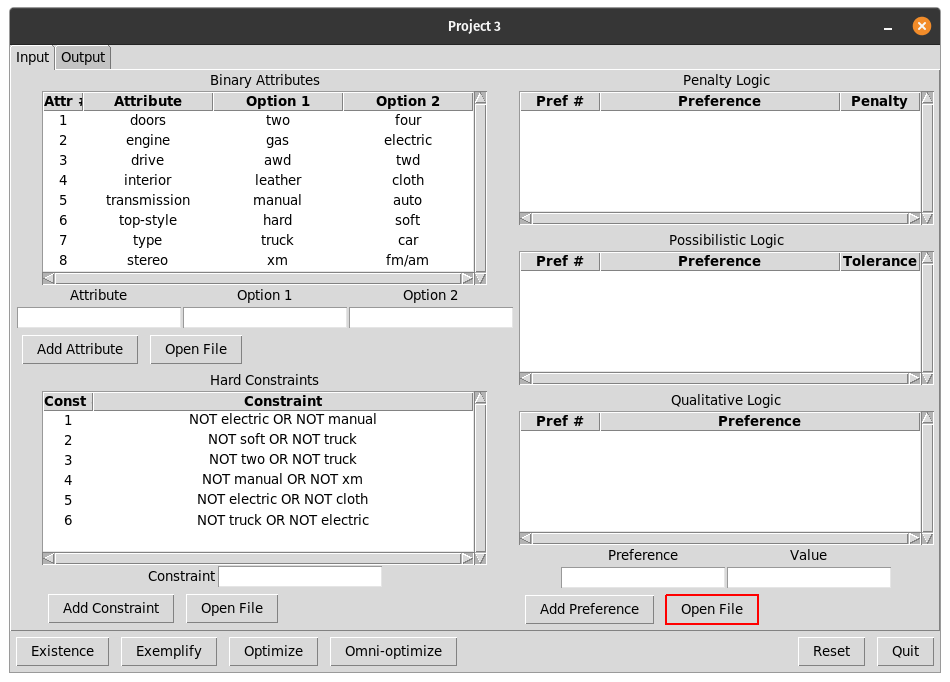
\includegraphics[scale=0.3,trim=1cm 1cm 1cm 1cm]{input_preferences}
\caption{Screenshot of selecting preference logics from a file}
\end{center}
\end{figure}
\vspace{-2.5em}
\item [Step 2:] Select the desired file (preferences$\_$test.txt for this example) and click \textbf{"Open"}.
\begin{figure}[H]
\begin{center}
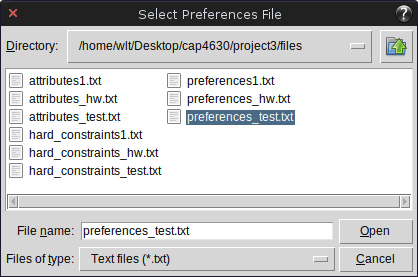
\includegraphics[scale=0.3,trim=1cm 1cm 1cm 1cm]{select_preferences}
\caption{Screenshot of selecting a preference logics text file}
\end{center}
\end{figure}
\vspace{-2.5em}
\item [Result:] The contents of the file will be displayed in the \textbf{three Preference Logics tables}
\begin{figure}[H]
\begin{center}
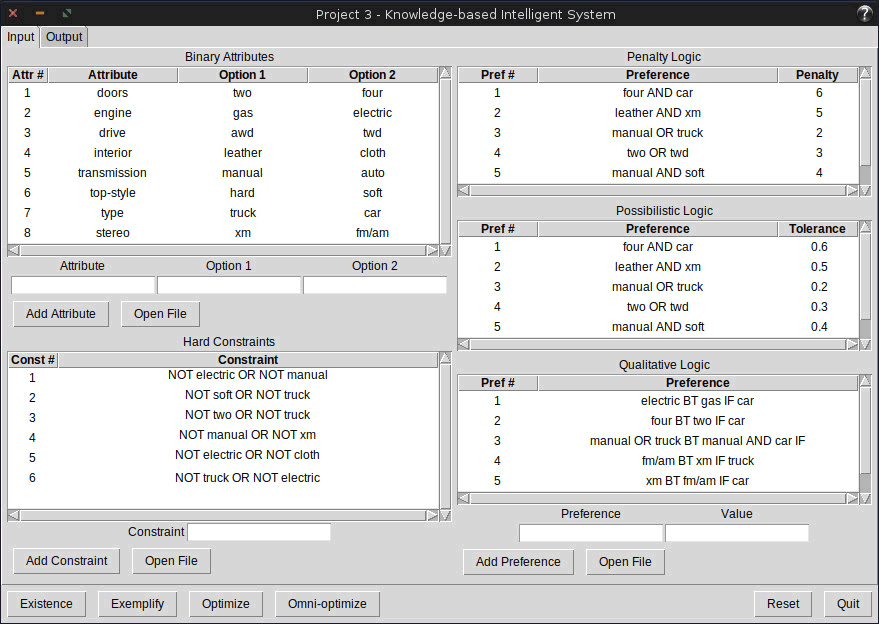
\includegraphics[scale=0.3,trim=1cm 1cm 1cm 1cm]{preferences_imported}
\caption{Screenshot of preference logics loaded from file}
\end{center}
\end{figure}
\vspace{-2.5em}
\end{description}


\chapter{Output}
\section{Existence of Feasible Objects}
The following steps demonstrate the existence of feasible objects functionality of the program.\\

\begin{description}[leftmargin=4em]
\item [Step 1:] Click the \textbf{"Existence"} button
\begin{figure}[H]
\begin{center}
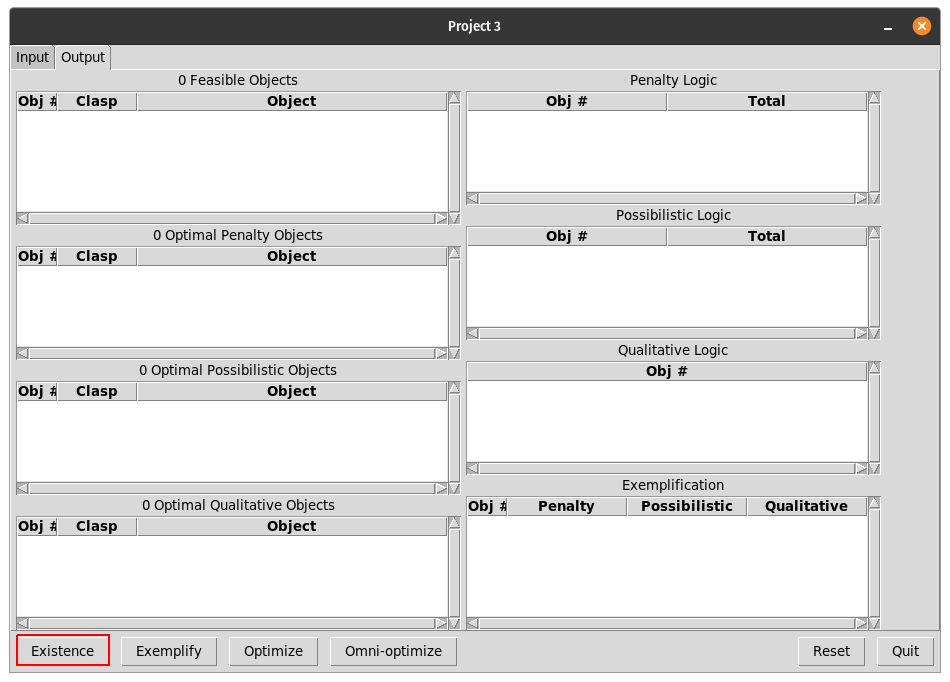
\includegraphics[scale=0.3,trim=1cm 1cm 1cm 1cm]{existence}
\caption{Screenshot of clicking the existence button}
\end{center}
\end{figure}
\vspace{-2.5em}
\item [Result:] All feasible objects will be displayed in the \textbf{feasible objects table} on the output tab, along with the total number of feasible objects. The output tab will be auto-focused on button click if on input tab when the button is clicked.
\begin{figure}[H]
\begin{center}
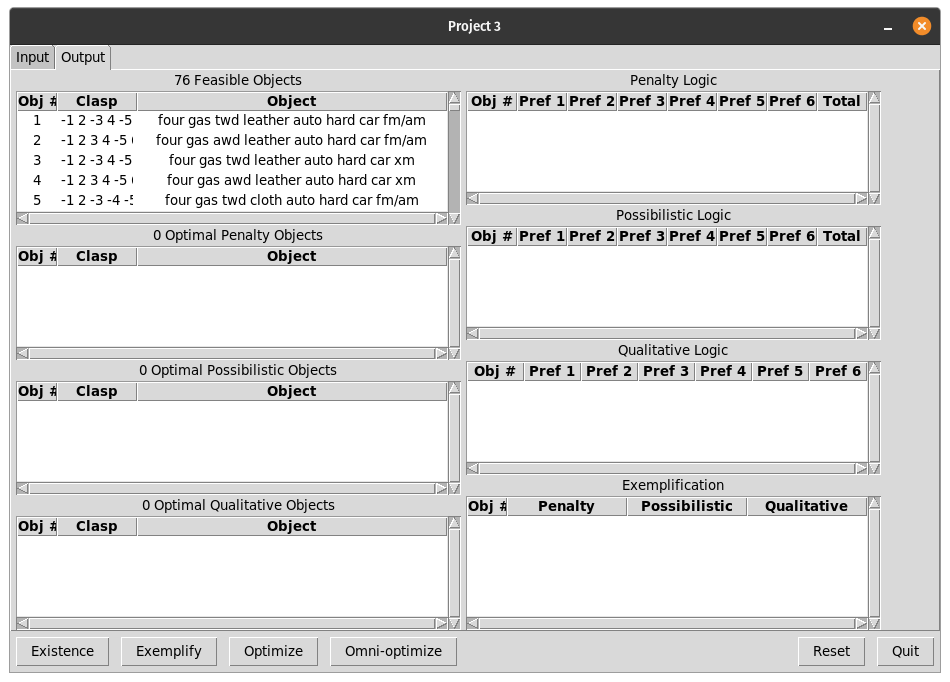
\includegraphics[scale=0.3,trim=1cm 1cm 1cm 1cm]{post_existence}
\caption{Screenshot of feasible objects output in table}
\end{center}
\end{figure}
\vspace{-2.5em}
\end{description}

\textbf{Note:} \\
Repetitive clicks of the existence button will always generate the same output in the table.

\newpage
\section{Exemplification}
\vspace{.75em}
The following steps demonstrate the exemplification functionality of the program. \\
Comparing two random feasible objects based on each of the three preference logics.\\

\begin{description}[leftmargin=4em]
\item [Step 1:] Click the \textbf{"Exemplify"} button
\begin{figure}[H]
\begin{center}
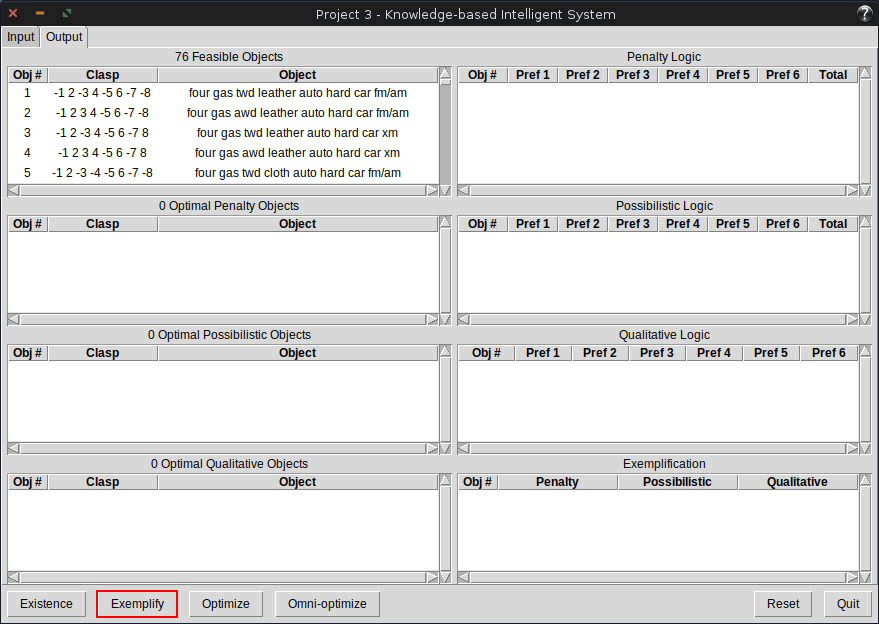
\includegraphics[scale=0.3,trim=1cm 1cm 1cm 1cm]{exemplify}
\caption{Screenshot of clicking the exemplify button}
\end{center}
\end{figure}
\vspace{-2.5em}
\item [Result:] The Penalty Logic, Possiblistic Logic, and Qualitative Choice Logic tables will be populated with the necessary underlying data used for exemplification. The \textbf{exemplification table} shows which objects are preferred for based on each logic.
\begin{figure}[H]
\begin{center}
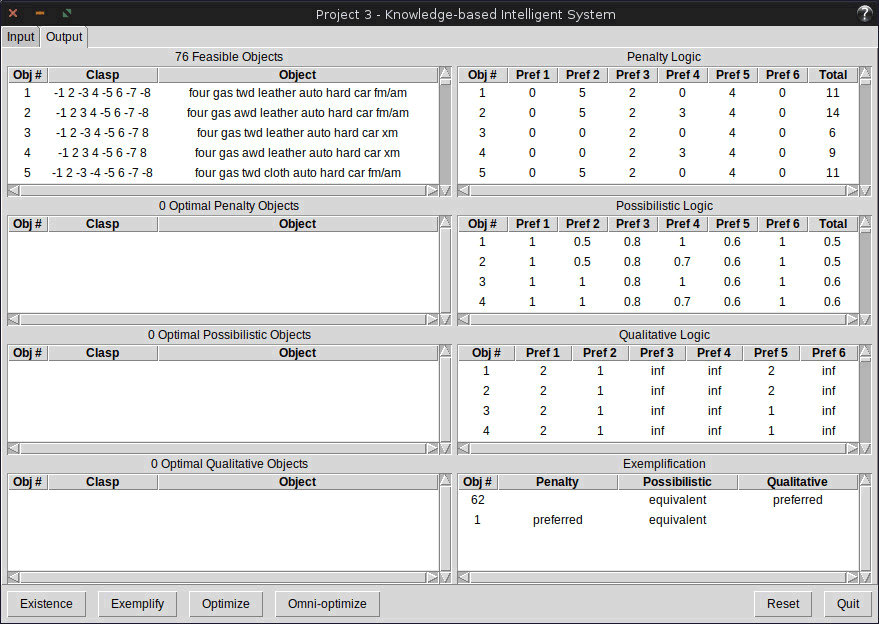
\includegraphics[scale=0.3,trim=1cm 1cm 1cm 1cm]{post_exemplify}
\caption{Screenshot of exemplification output in table}
\end{center}
\end{figure}
\vspace{-2.5em}
\end{description}
\textbf{Note:} \\
Repetitive clicks of the exemplify button will compare two different random feasible objects and generate different output in the table.

\newpage
\section{Optimization}
The following steps demonstrate the optimization functionality of the program. \\
Showing a optimal feasible object based on each of the three preference logics.\\

\begin{description}[leftmargin=4em]
\item [Step 1:]  Click the \textbf{"Optimize"} button
\begin{figure}[H]
\begin{center}
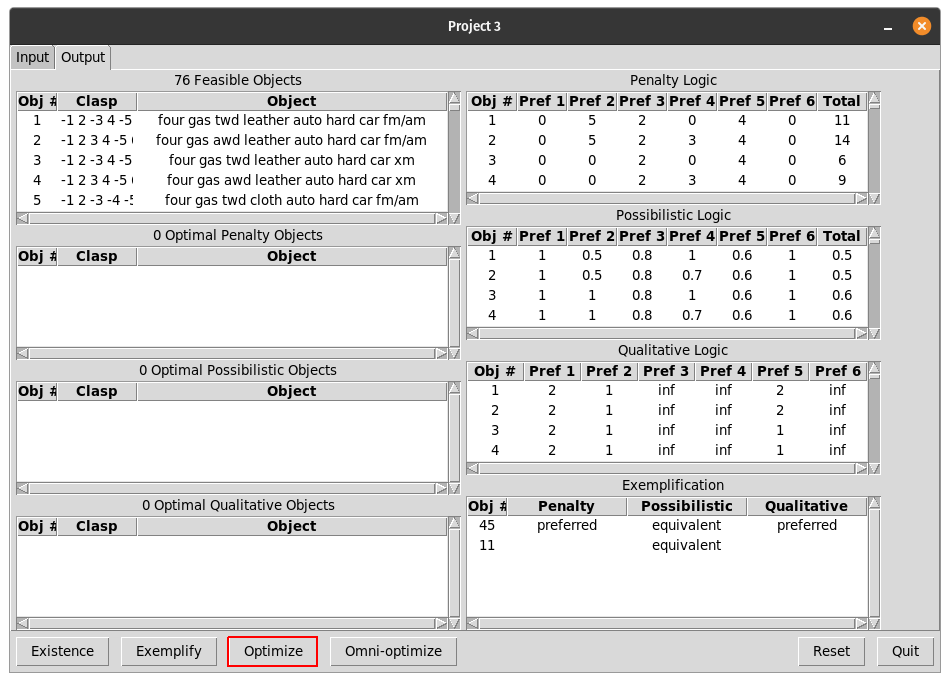
\includegraphics[scale=0.3,trim=1cm 1cm 1cm 1cm]{optimize}
\caption{Screenshot of clicking the optimize button}
\end{center}
\end{figure}
\vspace{-2.5em}
\item [Result:] The \textbf{Optimal Penalty Objects, Optimal Possiblistic Objects, and Optimal Qualitative Objects tables} will be populated with a single optimal object based on each logic.
\begin{figure}[H]
\begin{center}
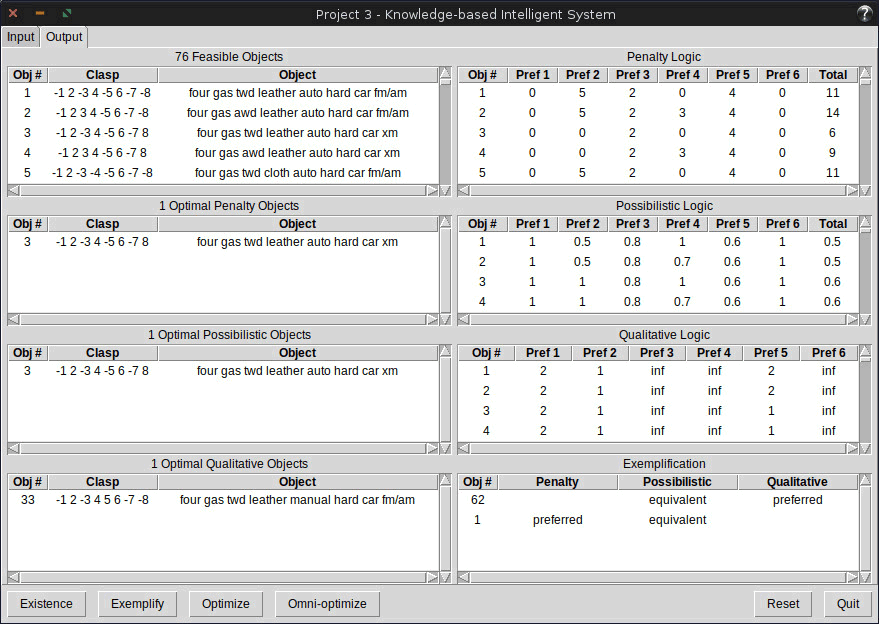
\includegraphics[scale=0.3,trim=1cm 1cm 1cm 1cm]{post_optimize}
\caption{Screenshot of optimization output in tables}
\end{center}
\end{figure}
\vspace{-2.5em}
\end{description}

\textbf{Note:} \\
Repetitive clicks of the optimize button will always generate the same output in the tables.

\newpage
\section{Omni-Optimization}
The following steps demonstrate the omni-optimization functionality of the program. \\
Showing all optimal feasible objects based on each of the three preference logics.\\

\begin{description}[leftmargin=4em]
\item [Step 1:]  Click the \textbf{"Omni-Optimize"} button
\begin{figure}[H]
\begin{center}
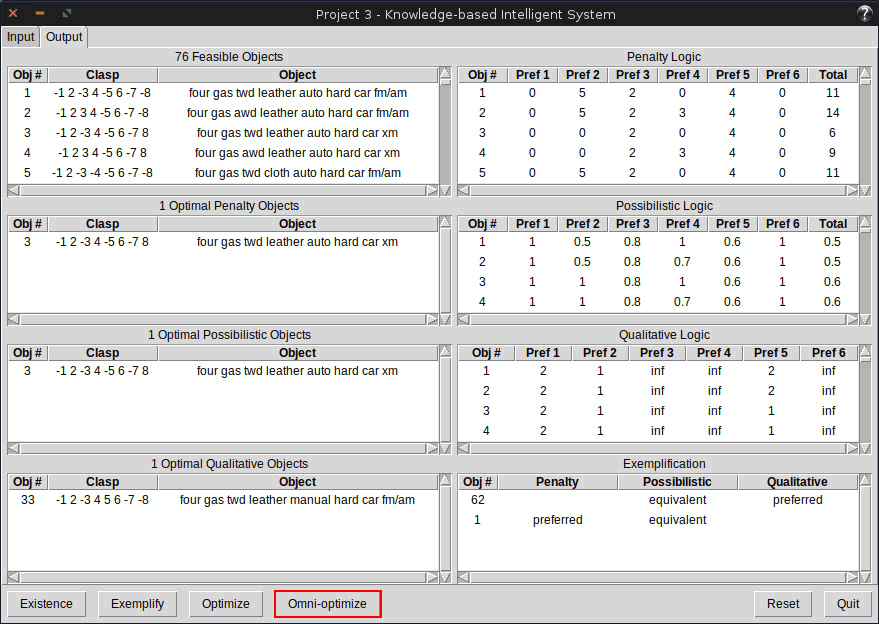
\includegraphics[scale=0.3,trim=1cm 1cm 1cm 1cm]{omni-optimize}
\caption{Screenshot of clicking the omni-optimize button}
\end{center}
\end{figure}
\vspace{-2.5em}
\item [Result:] The \textbf{Optimal Penalty Objects, Optimal Possiblistic Objects, and Optimal Qualitative Objects tables} will be populated with optimal objects based on each logic, along with the total number of optimal objects for each preference.
\begin{figure}[H]
\begin{center}
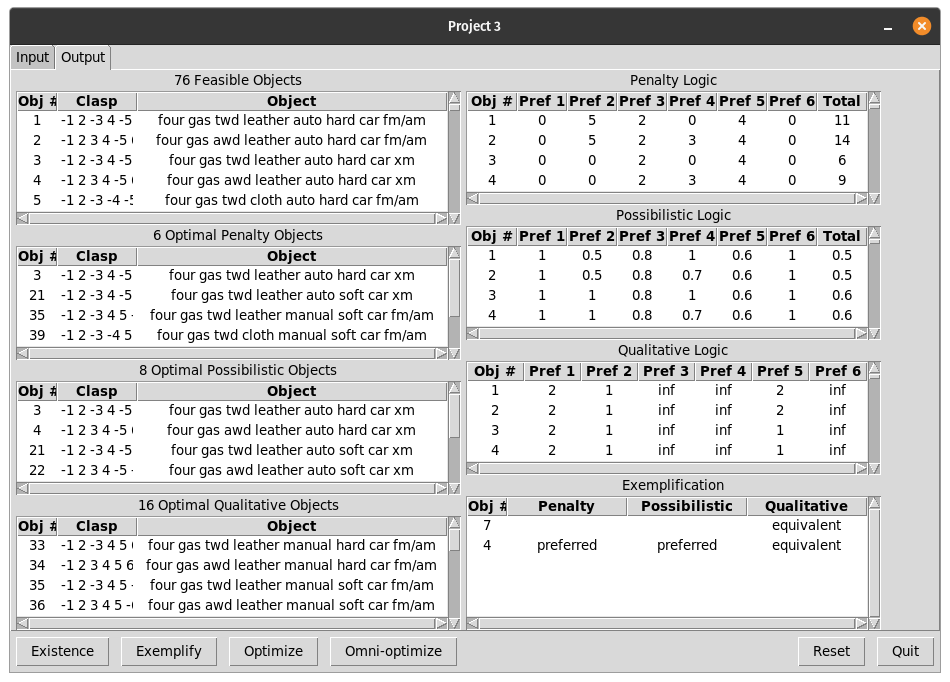
\includegraphics[scale=0.3,trim=1cm 1cm 1cm 1cm]{post_omni-optimize}
\caption{Screenshot of omni-optimization output in tables}
\end{center}
\end{figure}
\vspace{-2.5em}
\end{description}

\textbf{Note:} \\
Repetitive clicks of the omni-optimize button will always generate the same output in the tables.

\newpage
\chapter{Reset}
Steps to reset all tables and fields to their default empty state.\\

\begin{description}[leftmargin=4em]
\item [Step 1:]  Click the \textbf{"Reset"} button
\end{description}
\begin{figure}[H]
\begin{center}
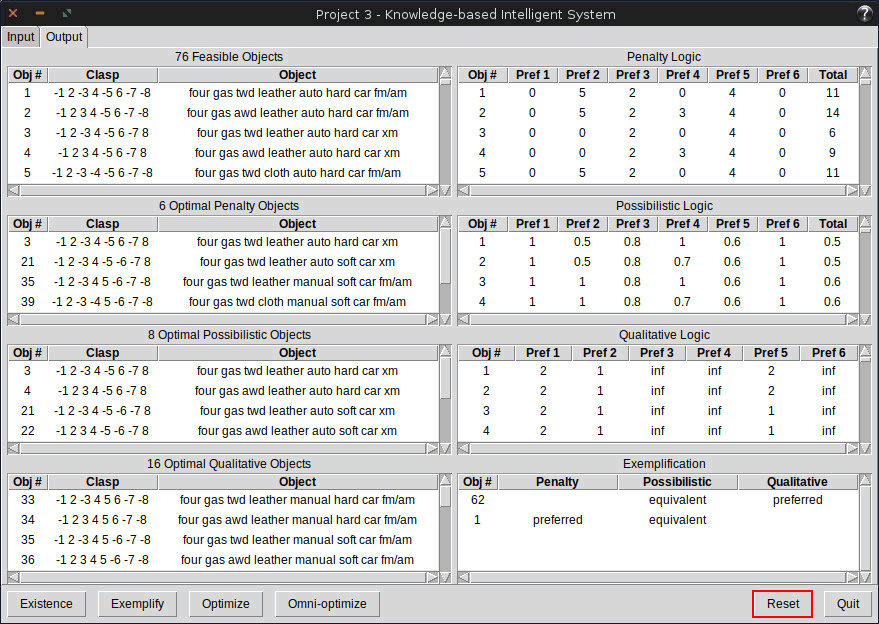
\includegraphics[scale=0.3,trim=1cm 1cm 1cm 1cm]{reset}
\caption{Screenshot of populated output tab}
\end{center}
\end{figure}
\vspace{-2.5em}
\begin{description}[leftmargin=4em]
\item [Result:] All tables have been cleared, and Penalty, Possibilitic and Qualitative tables have been reset to their default columns.
\end{description}
\begin{multicols}{2}
\begin{figure}[H]
\begin{center}
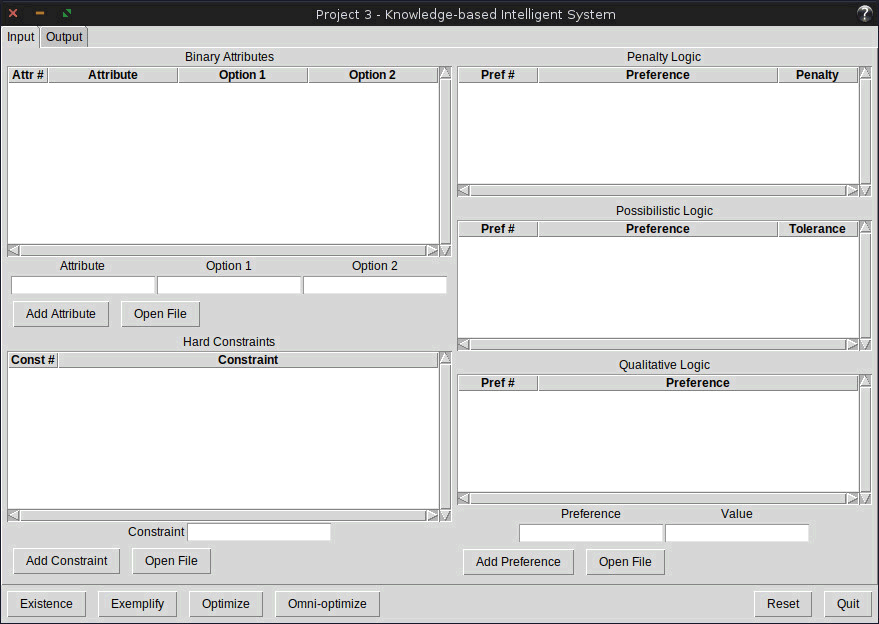
\includegraphics[scale=0.25,trim=1cm 1cm 1cm 1cm]{input_start}
\caption{Screenshot of input tab after reset}
\end{center}
\end{figure}
\begin{figure}[H]
\begin{center}
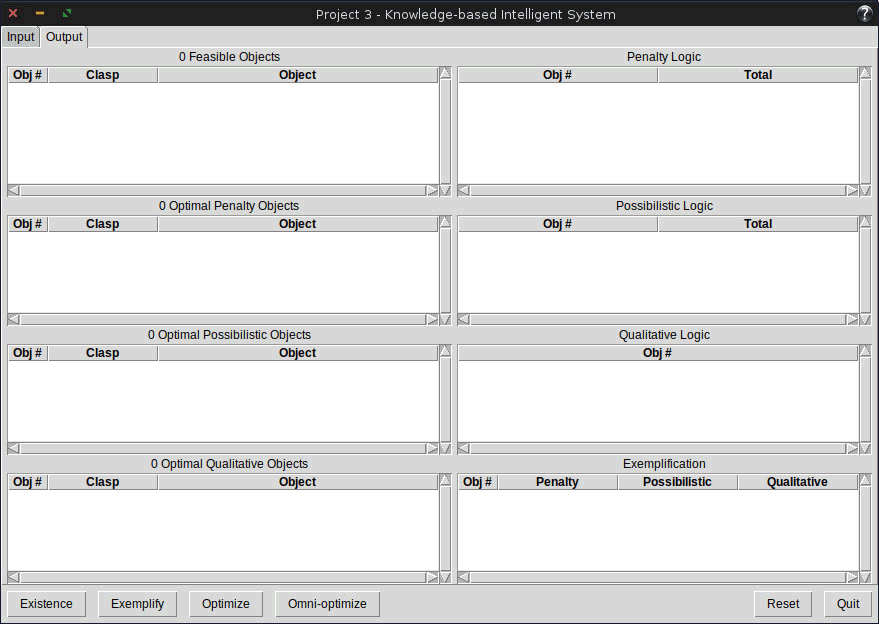
\includegraphics[scale=0.25,trim=1cm 1cm 1cm 1cm]{output_start}
\caption{Screenshot of output tab after reset}
\end{center}
\end{figure}
\end{multicols}

\newpage
\chapter{Quit}
Steps to quit the program.\\

\begin{description}[leftmargin=4em]
\item [Step 1:]  Click the \textbf{"Quit"} button
\end{description}
\begin{figure}[H]
\begin{center}
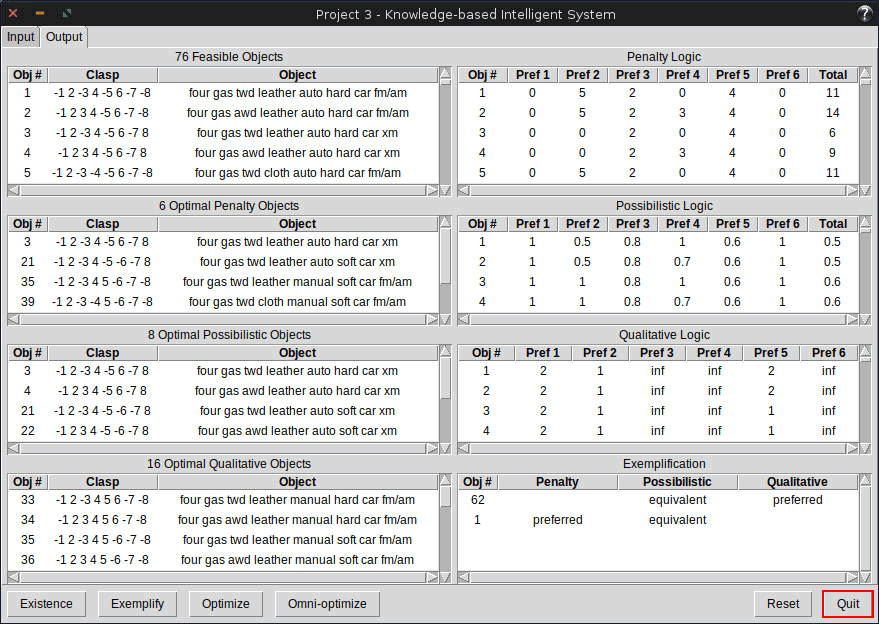
\includegraphics[scale=0.3,trim=1cm 1cm 1cm 1cm]{quit}
\caption{Screenshot of program before quit button click}
\end{center}
\end{figure}

\end{document}